\section{Cuestionario} 
\vspace{\baselineskip}
5.1 Los valores introducidos al archivo sysctl.conf ¿que representan?

\vspace{\baselineskip}

{\bfseries fs.suid\_dumpable}
\\
\\

{\bfseries fs.aio-max-nr}
\\
\\

{\bfseries fs.file-max}
\\
\\

{\bfseries kernel.shmmni}
\\
\\

{\bfseries  kernel.sem}
\\
\\Los semáforos actúan como banderas para la memoria compartida. Los semáforos se activan o desactivan. Cuando un proceso de Oracle accede al SGA en la memoria compartida, busca un semáforo para esa porción de memoria. \\
\\
\\Los valores para los semáforos representan lo siguiente:\\
\\•	semmsl : el número de semáforos por conjunto
\\•	semmns : el número total de semáforos disponibles
\\•	semopm : el número de operaciones que se pueden realizar por llamada de semáforo
\\•	semmni : el número máximo de segmentos de memoria compartida disponibles en el sistema
\\

{\bfseries  net.ipv4.ip\_local\_port\_range}
\\
\\Define el rango de puertos locales que utilizan TCP y UDP para elegir el puerto local. El primer número es el primero, el segundo el último número de puerto local. \\
\\Si es posible, es mejor que estos números tengan una paridad diferente, es decir, uno par y uno impar. 
\\
	\begin{center}
		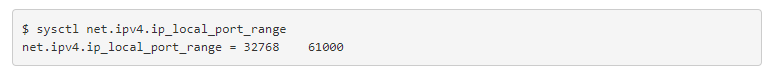
\includegraphics[width=17cm]{./Imagenes/c} 
	\end{center} 

{\bfseries  net.core.rmem\_default}
\\
\\Define el rango de puertos locales que utilizan TCP y UDP para elegir el puerto local. El primer número es el primero, el segundo el último número de puerto local. \\
\\Si es posible, es mejor que estos números tengan una paridad diferente, es decir, uno par y uno impar. 
\\
	\begin{center}
		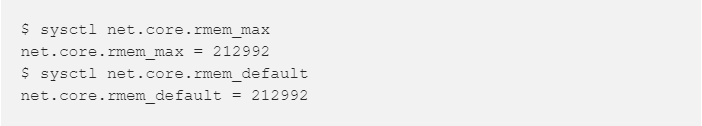
\includegraphics[width=17cm]{./Imagenes/t} 
	\end{center} 

{\bfseries  net.core.rmem\_max}
\\
\\Esto establece el tamaño máximo del búfer de recepción del sistema operativo para todos los tipos de conexiones.
\\
\\La configuración de net.core.rmem\_max define el tamaño máximo del búfer de socket de recepción en bytes.\\
\\
\\Hay algunas configuraciones diferentes que parecen ser muy similares. Puede ver que en Ubuntu 15.04 (3.18.0-13-generic) el valor predeterminado para net.core.rmem\_max es 212992. En este caso, los valores predeterminado y máximo son los mismos. Elevar este valor a un valor mayor aumentará el tamaño del búfer, pero esto puede tener efectos desagradables en términos de "acumulación de búfer". \\
	\begin{center}
		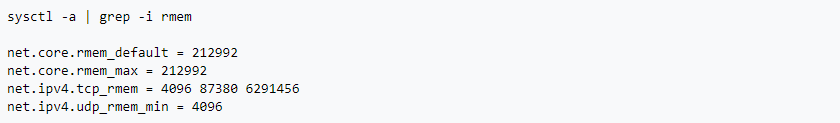
\includegraphics[width=17cm]{./Imagenes/s} 
	\end{center} 


{\bfseries  net.core.wmem\_default}
\\
\\Esto establece el tamaño del búfer de envío del sistema operativo predeterminado para todos los tipos de conexiones.
\\

{\bfseries  net.core.wmem\_max}
\\
\\Esto establece el tamaño del búfer de envío del sistema operativo predeterminado para todos los tipos de conexiones.
\\
\\La configuración de net.core.wmem\_max define el tamaño máximo del búfer de socket de envío en bytes.
\\
\\
Puede ver que en Ubuntu 15.04 (3.18.0-13-generic) el valor predeterminado para net.core.wmem\_max es 212992, que es del mismo tamaño que rmem\_max. Si aumenta esto a un valor mayor, aumentará el tamaño del búfer de envío.\\
\\
	\begin{center}
		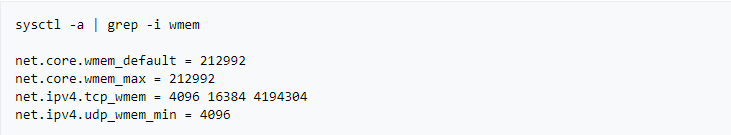
\includegraphics[width=17cm]{./Imagenes/p} 
	\end{center} 

5.2 ¿Con qué usuario(s) puedo conectarme al servidor a través del Administrador
Empresarial?
	\begin{center}
		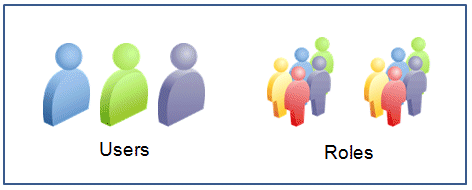
\includegraphics[width=13cm]{./Imagenes/users-oracle} 
	\end{center} 

	Los datos del login que se han utilizado para ingresar al Administrador Empresarial con:

	\begin{center}
		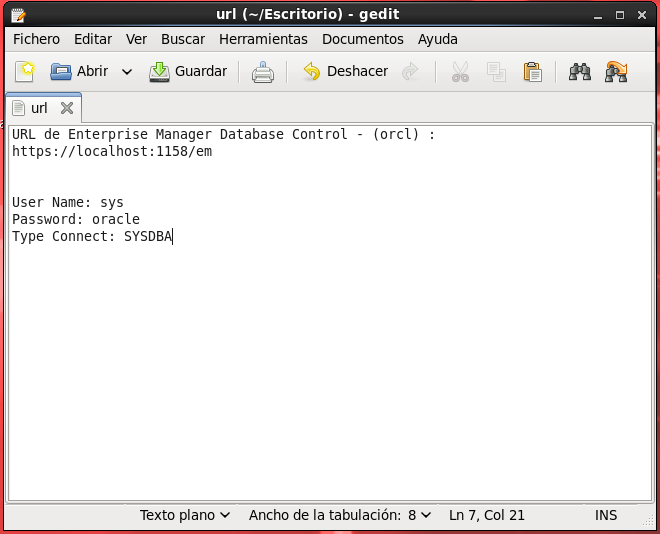
\includegraphics[width=15cm]{./Imagenes/94} 
	\end{center}

\vspace{\baselineskip}

5.3 Capture una imagen de pantalla del navegador con el Administrador Empresarial, con el nombre de su servidor e iniciada la sesión del usuario SYS.\\
\\
\\Para verificar de que la instalación ha sido exitosa, iniciar un navegador de Internet (Mozilla u otro similar), e introducir la dirección electrónica. Si todo es correcto aparecerá la interfaz de inicio de sesión de la herramienta Enterprise Manager (Administrador Empresarial) de Oracle.\\
\begin{center}
	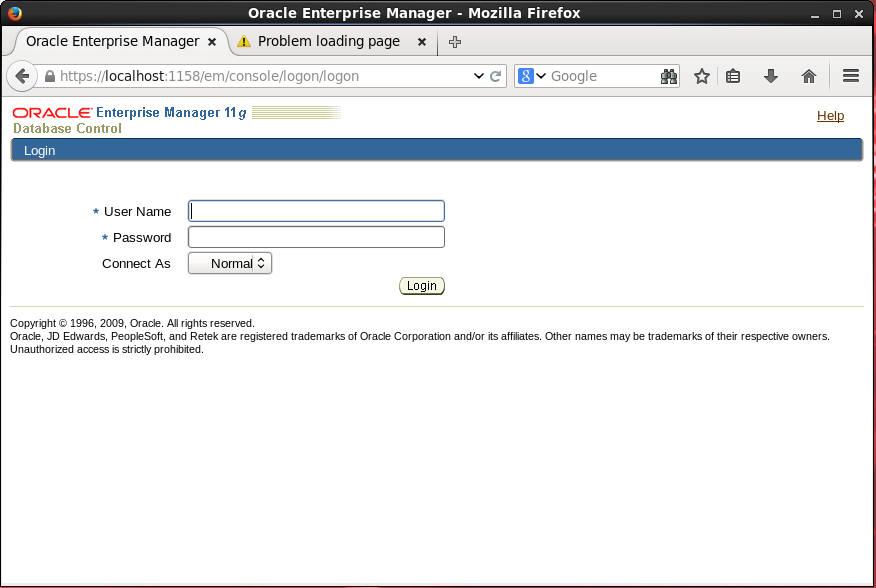
\includegraphics[width=16cm]{./Imagenes/91} 
\end{center}

Pero, si aparece la siguiente advertencia. para lo cual debemos ir a la Opcion I Understand the Risks
\begin{center}
	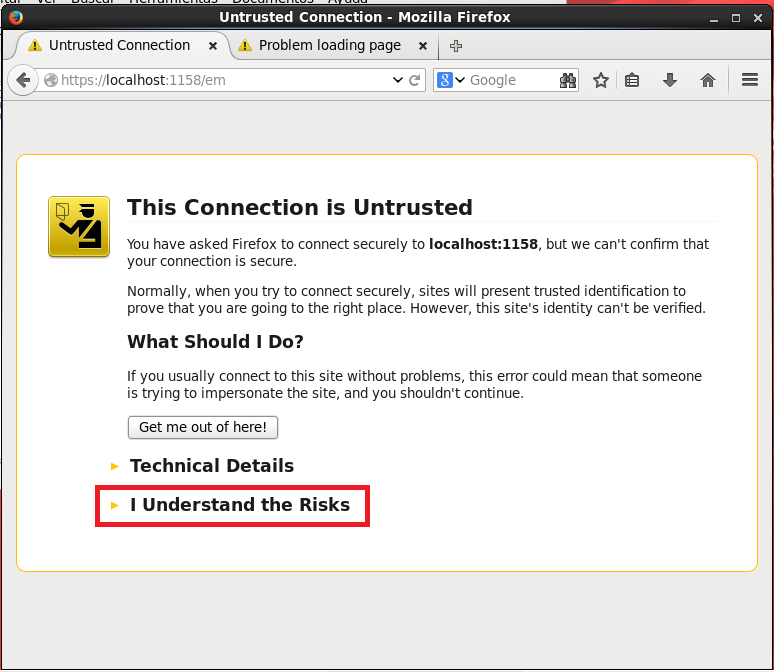
\includegraphics[width=15cm]{./Imagenes/88} 
\end{center}

Lo cual nos desglosara un comunicado, el cual presionamos el boton Add Exception
\begin{center}
	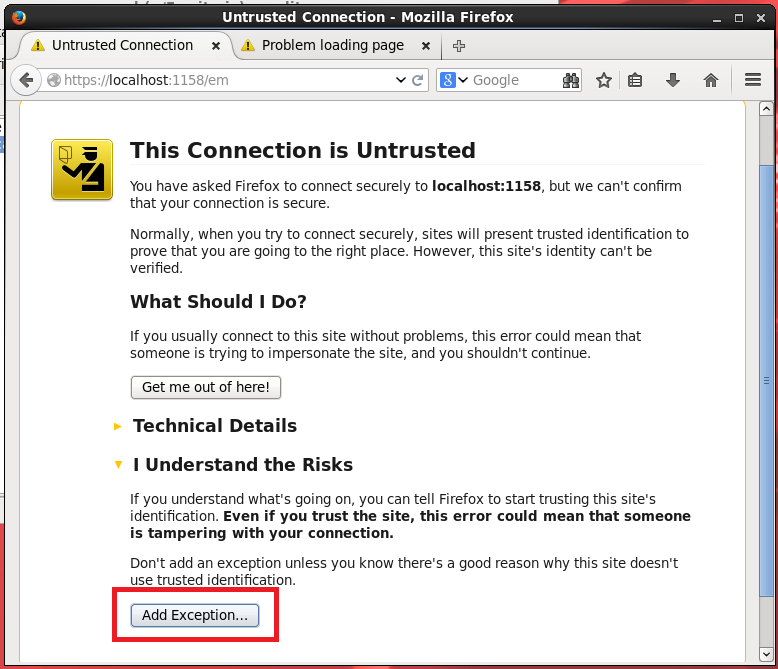
\includegraphics[width=15cm]{./Imagenes/89} 
\end{center}

Nos aparecera una nueva ventana de Advertencia donde presionaremos Confirm Security Exception
\begin{center}
	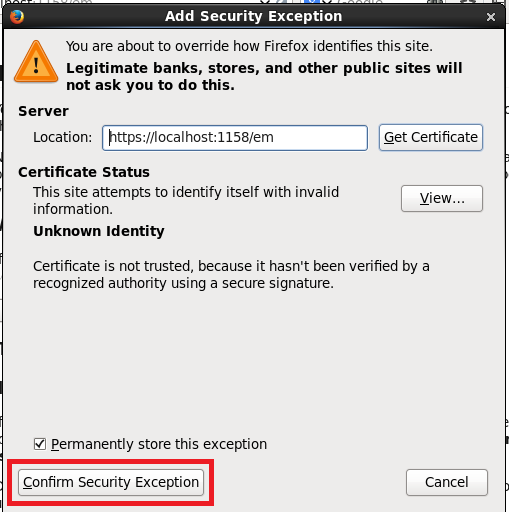
\includegraphics[width=10cm]{./Imagenes/90} 
\end{center}

Ya al culminar estos pasos podremos visualizar nuestra pagina de Login, donde podremos colocar nuestros datos
\begin{center}
	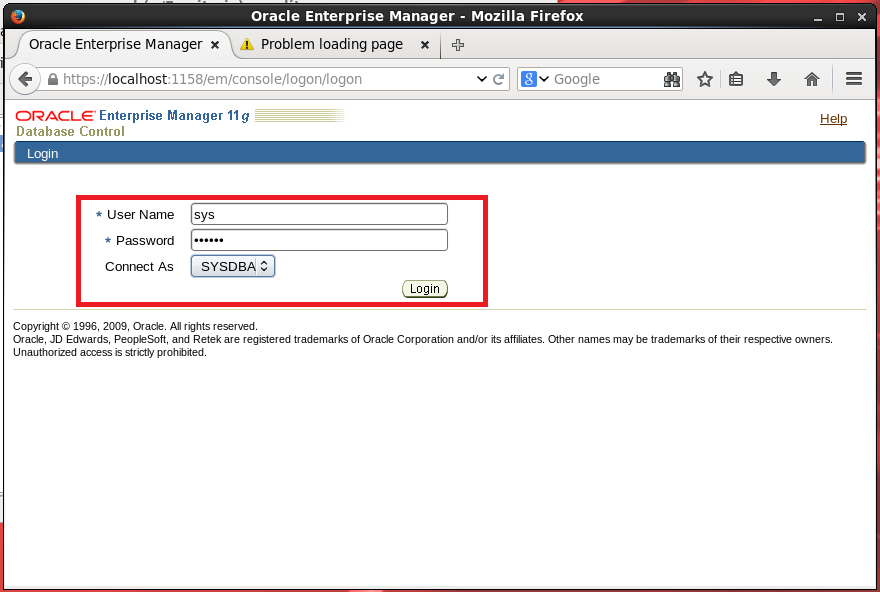
\includegraphics[width=15cm]{./Imagenes/92} 
\end{center}

Y cuando ingresemos nos aparecera la siguiente pagina de inicio
\begin{center}
	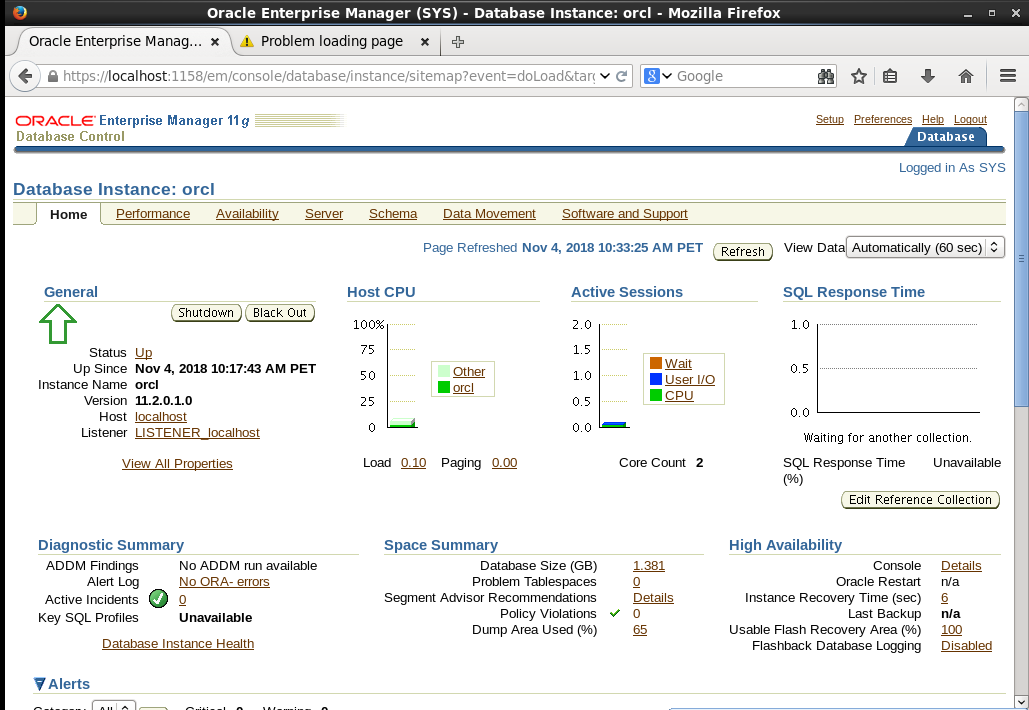
\includegraphics[width=15cm]{./Imagenes/93} 
\end{center}

Para no olvidarnos, es bueno mantener anotado la Url y los datos del Login.
\begin{center}
	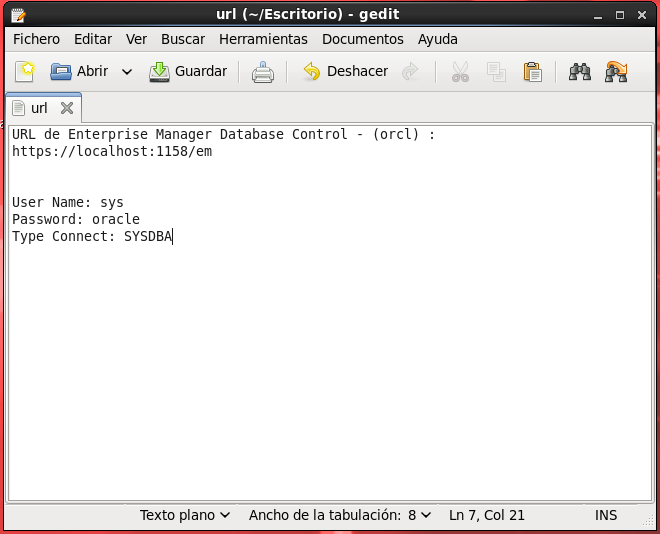
\includegraphics[width=15cm]{./Imagenes/94} 
\end{center}

